\documentclass[]{article}
\usepackage[koi8-r]{inputenc}
\usepackage{geometry}
\usepackage[pdftex]{graphicx}
\usepackage{wrapfig}
\graphicspath{{../images/}}
\DeclareGraphicsExtensions{.png}
%opening
\title{Astrometric Observations of the Main Uranian Satellites at the Pulkovo Observatory in 2007 -- 2016}
\author{Ershova A. P., Roschina E. A., Izmailov I. S.}
\geometry{left=2.5cm}
\geometry{right=2.5cm}
\geometry{top=2cm}
\geometry{bottom=2cm}
\begin{document}

\maketitle

\begin{abstract}
The results of observations of uranian satellites obtained with the Pulkovo Observatory 26-inch refractor in 2007 -- 2016 were presented. Almost 7000 CCD frames were analysed. The UCAC4 catalog was used as an astrometric calibrator. Coordinates of Uranus were determined indirectly with the satellites' positions and their ephemeris relative to the planet. The O-C differences were calculated for each object using the INPOP13c planetary theory and Lainey's theory of the satellites' motion. The mean values of the standard errors of (O-C) are within 0.02 to 0.07 arcsec. (O-C) absolute values are less than 0.5 arcsec. It is in a good agreement with ephemeris.
\end{abstract}

\section{Introduction}
High-precision theories of motion of the major planets and their satellites are necessary for researches of the Solar System formation and evolution, and for providing the ephemeridae for the future space missions. Construction of the theories requires an extensive observational material (Emel'yanov, 2009).\par

In the twentieth century photographic observations of Uranus were performed at the Pulkovo Observatory (Kiseleva, Khrutskaya, 2007). Coordinates of the planet were determined with respect to the reference stars directly, uranian satellites were inaccessible for the photographic method.\par

CCD-observations of Uranus have been started in 2007. The CCD-images of four main uranian satellites (Ariel, Umbriel, Titania and Oberon) are available for robust determination of positions. �Final astrometric accuracy of the satellites' observations is similar to the positional precision presented in several recent investigations (Camargo et al., 2015, Khovrichev, 2009). �The fifth main satellite of Uranus (Miranda) is usually located within small angular distant from the planet (within bright part of scattered-light halo caused by Uranus). Therefore its images could not be correctly approximated.\par

The first results of observations of uranian satellites with CCD-camera and 26-inch refractor in Pulkovo were published in 2013. (Roschina et al., 2013). Published observations covered period �2007 -- 2011. UCAC2 (Zacharias et al., 2010) was used as a reference catalog. Volume of observational data in current paper is significantly bigger. The resulted data sample contains satellites' positions taken from August 2007 to January 2016. The astrometric calibrations were performed with UCAC4 (Zacharias et al., 2013). This catalog provides significantly more stars in the field of view than UCAC2. It allows us to reach improvement of accuracy.

\section{Observations and mesaurements}

Current observations of Uranus are performed at the Pulkovo from the end of August to the beginning of January using the 26-inch refractor. The telescope is located at $59^o46' 15''$ north latitude, $30^o19'23''$ east longitude, altitude above the sea level is about 85 m. Aperture diameter of the telescope is 65 cm, focal length is 1041.3 cm, focal plane scale is 19''.80/mm in the center of image. The CCD camera FLI Pro Line 09000 is used. Size of the CCD matrix is 3056x3056 px, each of 12 $\mu$m. The field of view is $12'$x$12'$, the scale on the CCD frames is $0''.24$/px.\par

We obtained one normal position of each satellite per night in the case of availability of the satellite for observations. Each normal position was calculated on the basis of five individual positions measured independently. Exposure times were within the range from 3 s to 20 s. We stacked separate CCD-images to achieve optimal quality for approximation. The number of frames in stack procedure varies from 4 to 25. Satellites' motion on the celestial sphere during observation was approximated linearly, so the average moment of time for whole series and the normal position at this moment were determined.\par
Observations processing and coordinates measurement were performed with the IZMCCD software package (Izmailov et al., 1998). In case of distortion of �the satellite image by planet halo the procedure of approximation and subtraction of the halo signals was applied. For this purpose brightness distribution was approximated according to expression (\ref{2}). Coefficients $a, b, c, d$ were estimated by the least squares method, r is the distance to a certain point. Its coordinates were also selected by minimization of residuals.\par
\begin{equation}
\label{2}
I(r) = a + \frac{b}{r} + \frac{c}{r^2} + \frac{d}{r^3}
\end{equation}
We determined the photocenters of satellites and reference stars images using approximation of image profile with the Lorenz function (\ref{1}).


\begin{equation}
\label{1}
I(x,y) = \frac{C}{(1 + AR)^{\alpha}} + D
\end{equation}
\begin{center}
\begin{math}
R = \sqrt{(x-x_0)^2 + (1+B)(y-y_0)^2 +E(x-x_0)(y-y_0)}
\end{math}\\
\end{center}
where\par
\\
$I(x,y)$ -- brightness in the pixel which coordinates are ($x$, $y$)\par
$(x_0, y_0)$ -- coordinates of the photocenter\par
$\alpha$ --  determine the form of the curve, in our case $\alpha = 1.4$\par
$A$, $B$, $C$, $D$, $E$ -- parameters of model:\par
\vskip0.1cm

The Lorenz function parameters were obtained by solving an excess system of equations by the non-linear least squares method. Astrometric reduction was performed with the six-constant linear model. We taken into account the differential refraction effect of the first order. The UCAC4 (Zacharias et al., 2013) was adopted as a reference catalog. At least of 8 stars of the UCAC4 were located within field of view. The majority of frames were identified with more than 10 stars. \par
Errors of measurements were estimated on standard formulae.

\begin{math}
\sigma_x = \sqrt{\frac{\sum\limits_{k=1}^{N}(x_k-x_{mean})^2}{N-1}}; \varepsilon_x = \sigma_x/\sqrt{N}
\end{math}\\
where $x_k$ is an individual position, $x_{mean}$ is a normal position

We discarded data in the case of individual error of position was greater than critical value. This value was $0.''3$ in the case of Ariel and Umbriel and $0.''1$ in case of Titania and Oberon. Mean values of errors are shown in Table \ref{errors}.

\begin{table}[h!]
\caption{Mean errors of normal positions $\varepsilon$ and of individual positions $\sigma$ (arcsec)}
\label{errors}
\begin{center}
\begin{tabular}{|c|c|c|c|c|}
\hline
&Ariel&Umbriel&Titania&Oberon \\
\hline
$\varepsilon_\alpha (\sigma_\alpha)$&0.06 (0.11)&0.05 (0.09)&0.02 (0.03)&0.02 (0.03) \\
$\varepsilon_\delta (\sigma_\delta)$&0.06 (0.11)&0.07 (0.11)&0.02 (0.03)&0.02 (0.04) \\
\hline
\end{tabular}
\end{center}
\end{table}



\section{Results and comparing with theory}
Almost 7000 CCD images of Uranus and its satellites were collected from 2007 to 2016. Table \ref{number_of_points} contains the numbers of observational nights for each satellite. It corresponds to the number of normal positions obtained during the year. The quantities of the individual positions are shown in the parentheses.\par

\begin{table}
\caption{Numbers of the normal and the individual positions}
\label{number_of_points}
\begin{center}
\begin{tabular}{|c|c|c|c|c|c|c|c|c|c|}
\hline
 & 2007 & 2008 & 2009 & 2010 & 2011 & 2012 & 2013 & 2014 & 2015\\
\hline
Ariel & 0(0) & 0(0) & 3(15) & 0 (0) & 0(0) & 2 (10) & 2 (10) & 2 (10) & 7 (35)\\
Umbriel & 0(0) & 2 (10) & 4 (20) & 4 (20) & 4 (20) & 4 (20) & 14 (70) & 8 (40) & 11(55)\\
Titania & 3 (13) & 5 (25) & 11 (55) & 5 (25) & 15 (75) & 12 (60) & 19 (91) & 15 (74) & 21 (105)\\
Oberon & 4 (21) & 7 (35) & 11 (55) & 5 (25) & 18 (90) & 13 (65) & 18 (88) & 19 (94) & 21 (105) \\
\hline
\end{tabular}
\end{center}
\end{table}

Obtained normal positions are not evenly distributed over the period of observations. An increasing number of obtained positions is seen from 2007 to 2016. This effect was noticed in earlier work (Camargo et al., 2015). It is explained by change of the angle between the equatorial plane of Uranus and the tangent plane. In the beginning of observational span the equatorial plane of the planet (and also the satellites' orbital planes), was very close to perpendicular to the tangent plane. Therefore uranian satellites spent most of the time behind the planet or right in front of it, so their coordinates could not be determined with CCD observations. This angle decreased at the end of observational period. As a result the satellites' images became more available for CCD astrometric observations.\par
We would like to show this effect by calculating the K coefficient. Let K be a ratio of the number of normal positions obtained during an observational season to the number of nights in this season. The observational season is a period of time from the end of August to the beginning of January. �Figure (\ref{fig:K}) illustrates increasing of this ratio.\par

\begin{wrapfigure}[12]{r}{0.4\linewidth} 
\vspace{-4ex}
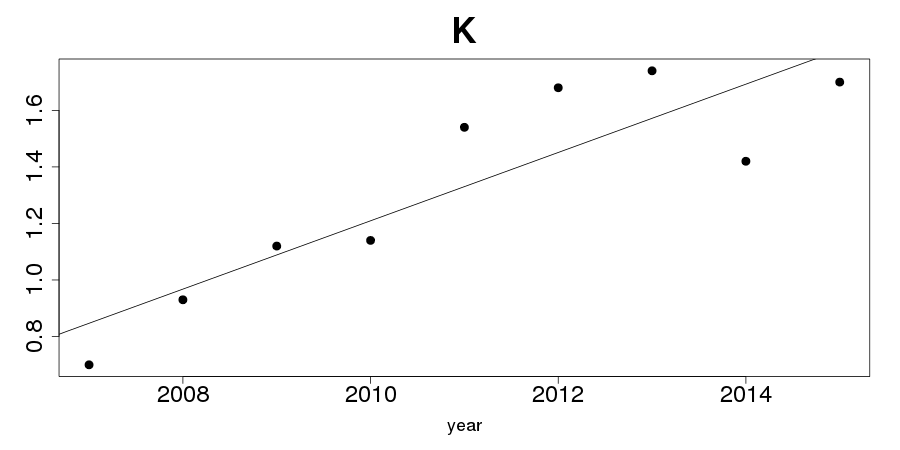
\includegraphics[width=\linewidth]{K}
\caption{{\footnotesize Ratio of the number of normal positions obtained during a season to the number of observational nights}}
\label{fig:K}
\end{wrapfigure}



Observed positions were compared with coordinates predicted with the planet motion theory INPOP13c (Fienga et al., 2014) and the Lainey's theory of uranian satellites' motion (Lainey, 2008). The ephemeridae were provided by the MULTI-SAT service (Emel'yanov and Arlot, 2008). We used the Lainey 2015 ephemeris available on the MULTI-SAT. This is an updated version of Lainey's theory.\par
Also positions of Uranus were determined with the positions of its satellites and ephemeris distances between them and the planet. Series of the O-C differences for each satellite and for the planet are shown on plots, the average O-C differences are in the Table \ref{mean_OC}.
Observations show a good agreement with theory.\par
\begin{table}
\begin{center}
\caption{Mean O-C differences}
\label{mean_OC}
\begin{tabular}{|c|c|c|c|c|c|}
\hline
& Ariel&Umbriel&Titania& Oberon & Uranus \\
\hline
Average $(O-C)_\alpha$ & 0.043 & 0.025 & -0.009 & -0.001 & 0.001\\
Average $(O-C)_\delta$ & -0.074 & -0.069 & -0.014 & -0.019 & -0.021\\
\hline
\end{tabular}
\end{center}
\end{table}

\newpage


\begin{figure}[h!]
\begin{minipage}[h]{0.49\linewidth}
\centering{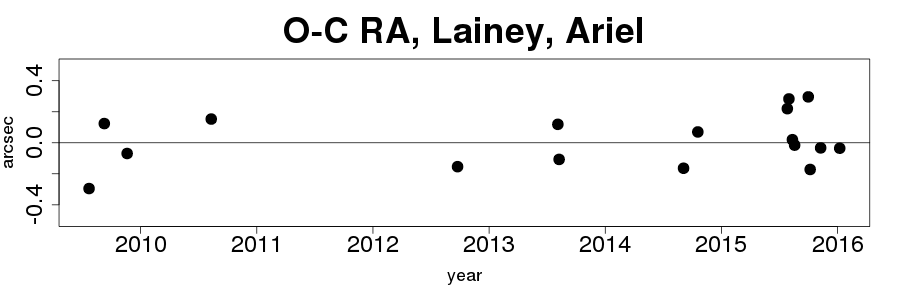
\includegraphics[width=1.0\linewidth]{Ariel_Lainey_RA}\\Ariel, $(O-C)_\alpha$}
\end{minipage}
\begin{minipage}[h]{0.49\linewidth}
\centering{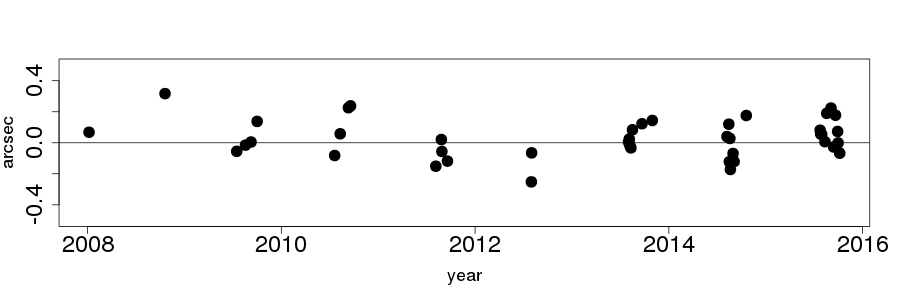
\includegraphics[width=1.0\linewidth]{Umbriel_Lainey_RA}\\Umbriel, $(O-C)_\alpha$}
\end{minipage}
\end{figure}
\begin{figure}[h!]
\begin{minipage}[h]{0.49\linewidth}
\centering{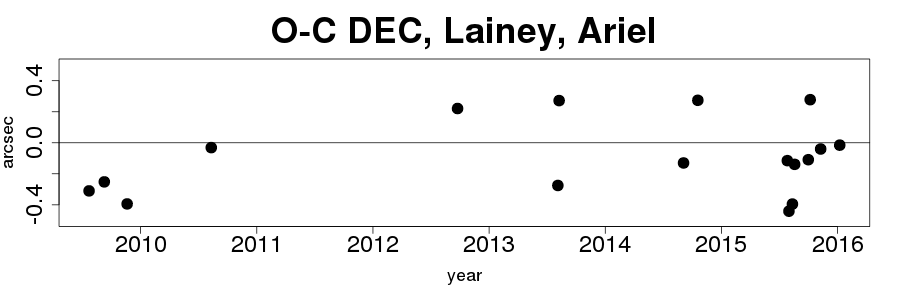
\includegraphics[width=1.0\linewidth]{Ariel_Lainey_DEC}\\Ariel, $(O-C)_\delta$}
\end{minipage}
\begin{minipage}[h]{0.49\linewidth}
\centering{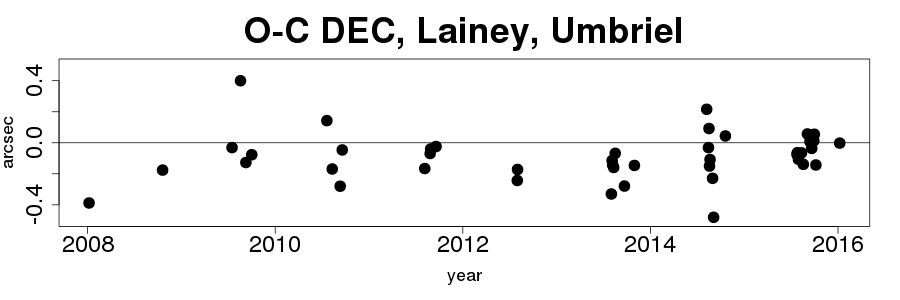
\includegraphics[width=1.0\linewidth]{Umbriel_Lainey_DEC}\\Umbriel, $(O-C)_\delta$}
\end{minipage}
\end{figure}


\begin{figure}[h!]
\begin{minipage}[h]{0.49\linewidth}
\centering{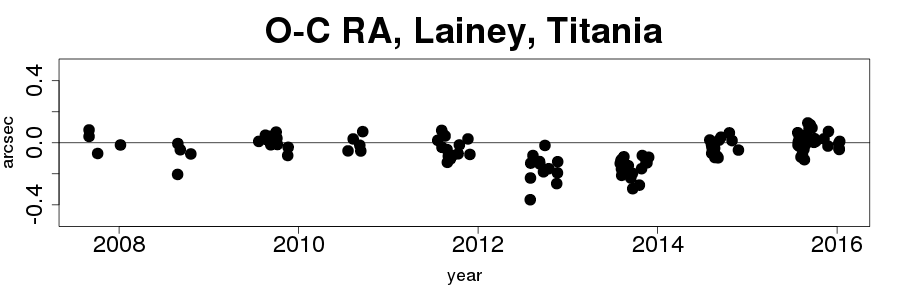
\includegraphics[width=1.0\linewidth]{Titania_Lainey_RA}\\Titania, $(O-C)_\alpha$}
\end{minipage}
\begin{minipage}[h]{0.49\linewidth}
\centering{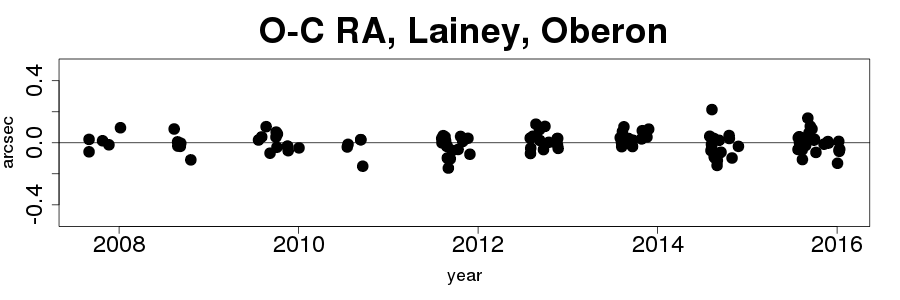
\includegraphics[width=1.0\linewidth]{Oberon_Lainey_RA}\\Oberon, $(O-C)_\alpha$}
\end{minipage}
\end{figure}
\begin{figure}[h!]
\begin{minipage}[h]{0.49\linewidth}
\centering{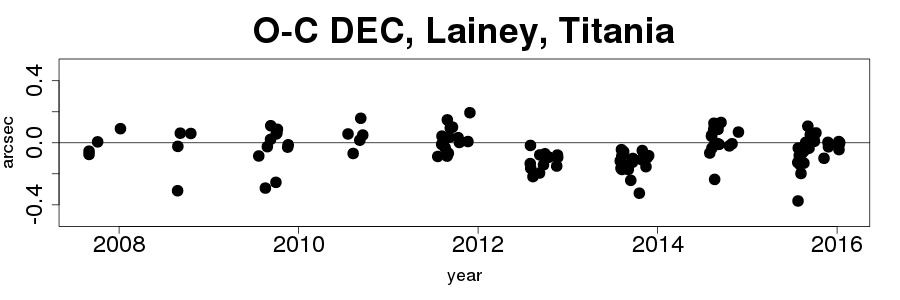
\includegraphics[width=1.0\linewidth]{Titania_Lainey_DEC}\\Titania, $(O-C)_\delta$}
\end{minipage}
\begin{minipage}[h]{0.49\linewidth}
\centering{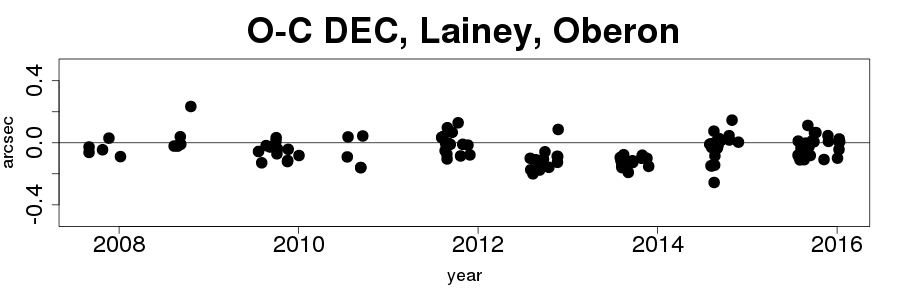
\includegraphics[width=1.0\linewidth]{Oberon_Lainey_DEC}\\Oberon, $(O-C)_\delta$}
\end{minipage}
\end{figure}





\section{Conclusion}
This paper has reported the results of uranian satellites' CCD observations performed at the Pulkovo Observatory with the 26-inch refractor in 2007 -- 2016. Results' analysis has demonstrated high-quality and the suitability of methods applied in this work. In particular the method of halo subtracting is useful for obtaining coordinates of inner satellites of Solar System planets and other small celestial bodies approaching bright objects in tangent plane. Observed positions of the main uranian satellites are usually close to ephemeris positions. The obtained normal positions are available in the Pulkovo database and in the CDS database.\par

\section{Acknowledgments}

The authors express their thanks to M. Yu. Khovritchev for his help in preparing the text of the paper.\\
This work was supported by the Presidium of RAS program no. 7. \par



\begin{thebibliography}{99}
\bibitem{1} \textquotedblleft Astrometric Observations of Satellites of Uranus Using 26-Inch Refractor in 2007--2011\textquotedblright, 2013, E. A. Roschina, I. S. Izmailov, T. P. Kiseleva
\bibitem{2}  \textquotedblleft Astrometry of the main satellites of Uranus: 18 years of observations\textquotedblright, 2015, J.I.B. Camargo, F. P. Magalhaes, R. Vieira-Martins, M. Assafin, F. Braga-Ribas, A. Dias-Oliveira,G. Benedetti-Rossi, A. R. Gomes-Junior, A. H. Andrei and D. N. da Silva Neto
\bibitem{7} M.Yu. Khovrichev, Astrometric observations of the Uranian satellites with the Faulkes telescope North in 2007 September, 2009
\bibitem{6} Izmailov I.S., Kiselev A.A., Kiseleva T.P., and Khrutskaya E.V., Using a CCD-camera in Pulkovo programs of observations of binary and multiple stars and satellites of major planets with the 26-inch refractor . Astron. Lett., 1998, vol. 24, no. 5, pp. 665-672.
\bibitem{3}  Izmccd is a software  packet for processing digital images of celestial objects, 2005, Izmailov, I.S., http://www.izmccd.puldb.ru/
\bibitem{4} Emel'yanov N.V., Precision of the ephemerides of outer planetary satellites, 2009, Planetary and Space Science
\bibitem{5} Emel'yanov N.V. and Arlot J.-E., The natural satellites ephemerides facility MULTI-SAT, Astron., Astrophis., 2008, vol. 487, pp. 759-765
\bibitem{8} Kiseleva T.P., Khrutskaya E.V., Pulkovo astrometric observations of bodies of the Solar System from 1898 to 2005: observational database, Solar. Syst. Res., 2007 vol. 41, no. 1, pp. 72-80
\bibitem{9} Zacharias, N.; Finch, C. T.; Girard, T. M.; Henden, A.; Bartlett, J. L.; Monet, D. G.; Zacharias, M. I., The Fourth US Naval Observatory CCD Astrograph Catalog (UCAC4), The Astronomical Journal, Volume 145, Issue 2, article id. 44, 14 pp. (2013)
\bibitem{10} Zacharias N., Finch C., Girard T., Hambly N., Wycoff G., Zacharias M.I., Castillo D., Corbin, T., DiVittorio, M.,Dutta,  S.,  Gaume,  R.,  Gauss,  S.,  Germain,  M., Hall,  D.,  Hartkopf,  W.,  Hsu,  D.,  Holdenried,  E., Makarov,  V.,  Martinez,  M.,  Mason,  B.,  Monet,  D., Rafferty, T., Rhodes, A., Siemers, T., Smith, D., Tilleman, T., Urban, S., Wieder, G., Winter, L., and Young, A., The third US Naval Observatory CCD Astrograph Catalog   (UCAC3), Astron.   J.,   2010,   vol.   139,   no.   6, pp. 2184?2199.
\bibitem{11} A. Fienga, H. Manche, J. Laskar, M. Gastineau, and A. Verma, 2014, INPOP new release: INPOP13c, arXiv:1405.0484
\bibitem{12} Lainey V.,	A new dynamical model for the Uranian satellites, 2008, Planetary and Space Science, Volume 56, Issue 14, p. 1766-1772
\end{thebibliography}






\end{document}
